This is illustrated in Figure~\ref{fig:proton_alignment}, notice that the distribution of protons into these two states is influenced by thermal energy and a slight majority align in the low-energy, parallel direction, resulting in an observable net magnetic moment (red arrow) usually denoted as equilibrium magnetization ($M_0$).

\begin{figure}[htb!]
	\centering
	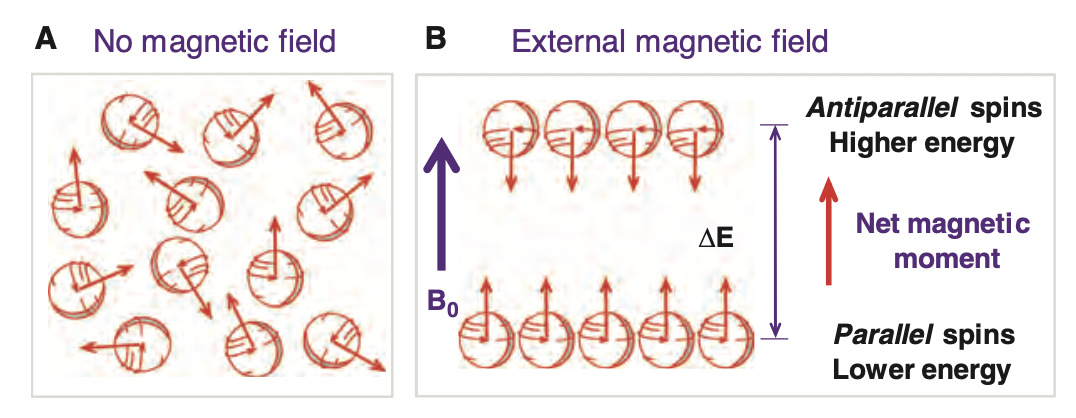
\includegraphics[width=\textwidth]{Assets/MRIproton.png}
	\caption[Proton alignment in a magnetic field]{Schematic illustration of how hydrogen protons ($^1$H) behave in the presence of a strong static magnetic field ($B_0$). 
		A: In the absence of a field, proton magnetic moments are randomly oriented, producing no net magnetization. 
		B: When exposed to $B_0$, protons align either parallel or antiparallel to the field. 
		From Bushberg, J.T., \textit{The Essential Physics of Medical Imaging} (2011) \cite{bushberg2011}.}
	\label{fig:proton_alignment}
\end{figure}


Depicted in Figure \ref{fig:protonPrecession}, the motion happens around the axis of the applied magnetic field due to the perpendicular torque they experience. 

\begin{figure}[htb!]
	\centering
	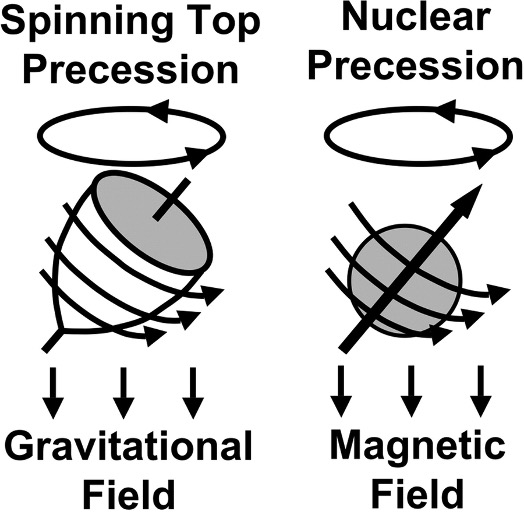
\includegraphics[width=0.55\linewidth]{Assets/protonPrecession.jpg}
	\caption[Analogy between proton spin precession and precession of a spinning top.]{Illustration of proton precession under a static magnetic field $B_0$ compared to that of a spinning top under gravity. Adapted from Pooley, R. A., \textit{Fundamental physics of MR imaging}, (2005) \cite{Pooley2005}.}
	\label{fig:protonPrecession}
\end{figure}